%Copyright (C) 2014 Sergio García Villalonga.

\subsection{Telèfon intel·ligent}

Per realitzar tant el mapa de potència de senyal com les proves s'ha fet servir un telèfon intel·ligent LG Nexus 4.

Aquest telèfon executa el sistema operatiu Android, sorgit al 2008 com alternativa lliure als sistemes per telèfons existents en la època, majoritàriament privatius. En un principi, va ser desenvolupat per la companyia Android Inc., i


\textit{Android} es un sistema operativo basado en \textit{Linux} desarrollado inicialment por Android Inc, i posteriorment per \textit{Google}. Se anunció en 2007 y el primer dispositivo que lo utilizó se lanzó en 2008. Se trata de un sistema operativo de código abierto, lo que ha provocado una gran adopción\footnote{De acuerdo con \url{http://gs.statcounter.com/\#mobile_os-ww-monthly-200812-201108} la adopción de Android ha aumentado significativamente desde su lanzamiento en 2008, en detrimento de otras plataformas como \textit{iOs} o \textit{Symbian}, siendo actualmente el sistema operativo móvil más utilizado \url{http://www.idc.com/prodserv/smartphone-os-market-share.jsp}.} Su naturaleza de código abierto ha hecho posible que no solo se utilice en telefonía móvil, sino que ha sido adaptado también para su funcionamiento en portátiles, \textit{tablets}, rellotges i ulleres intel·ligents, televisions, en sistemas de automóviles\footnote{Un proyecto está en marcha entre Google y General Motors para llevarse a cabo \url{http://www.theinquirer.es/2010/05/13/google-android-llegara-al-automovil-de-la-mano-de-general-motors.html}.} o de domótica\footnote{Por ejemplo el proyeto \textit{Android@Home} \url{http://www.engadget.com/2011/05/10/google-announces-android-at-home-framework/}.}. El sistema ofrece no solo las funciones básicas de un teléfono móvil como son las llamadas telefónicas o el envío de mensajes, sino que provee un entorno de desarrollo y unas herramientas para poder programar aplicaciones de propósito general. Además también provee mecanismos para que las aplicaciones se puedan comunicar entre sí y utilizar los servicios y recursos del teléfono. Estos recursos incluyen herramientas indispensables para el posicionamiento, tales como la brújula, acceleròmetre i gisroscopi.  \newline

La mayor desventaja de \textit{Android} es que, pese a que ha sido posible portarlo a plataformas muy diferentes al ser código abierto, este último hecho ha provocado que exista una gran variedad de dispositivos con diferentes tamaños, resoluciones de pantalla o con diferentes versiones del sistema operativo, hecho conocido como fragmentación. Este hecho provoca que ciertas aplicaciones que no tienen estos aspectos en cuenta no funcionen en todos los dispositivos ya que ciertas características no son compatibles hacia atrás. Pese a que esta última desventaja es común en otro software, en este caso el problema se acentúa ya que no siempre los fabricantes actualizan sus teléfonos al salir una nueva versión del sistema. La figura \ref{fig:Frangmentacion1} muestra esta tendencia.\newline

\begin{figure}[ht]
\begin{center}
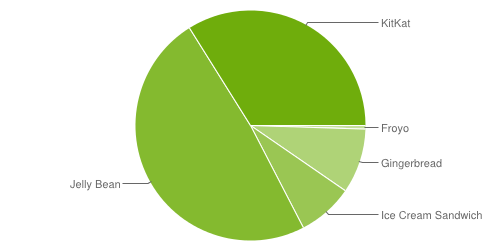
\includegraphics[width=10cm]{imatges/chart.png}
\caption{Gráfico que muestra la actual situación de la fragmentación de los dispositivos que utilizan Android. Fuente: \cite{android2}.}
\label{fig:Frangmentacion1}
\end{center}
\end{figure}

Por otro lado, centrándonos en las herramientas proporcionadas por \textit{Google} para desarrollar sobre \textit{Android}, podemos distinguir dos conjuntos. Primero, el más común y recomendado, el \textit{Android \textit{SDK}}. El \textit{Android \textit{SDK}} proporciona las herramientas estándar de programación a alto nivel que permiten desarrollar programas aprovechando los recursos del teléfono móvil. Está basado en Java y, de la misma manera que lo que ocurre con este lenguaje de programación, las aplicaciones se ejecutan sobre una máquina virtual llamada \textit{Dalvik}\cite{wiki4}. La principal diferencia con la manera de funcionar de Java, es que \textit{Android} ejecuta una máquina virtual Dalvik por cada aplicación. Ello permite encapsular las aplicaciones, permitiendo al sistema controlar mejor la seguridad o los recursos utilizados por cada aplicación.\newline

Pese a las ventajas y seguridad, no es la manera recomendada de realizar aplicaciones que necesiten una gran eficiencia en su ejecución. Para estas últimas se provee una serie de herramientas llamadas \textit{Android \textit{NDK}}. El \textit{Android \textit{NDK}} permite realizar programas en \textit{C} o \textit{C++} a un nivel mucho más bajo que las aplicaciones que utilizan el \textit{SDK}\cite{android1}, y que permiten ejecutar el código de manera más eficiente. Pero el poder acceder a recursos a bajo nivel (como por ejemplo, para reservar más memoria de la que permite el \textit{SDK}), hace que sea más inseguro programar mediante estas herramientas. Además, las librerías proporcionadas por el \textit{NDK} no son tan completas como las del \textit{SDK}, por lo que la programación es más limitada (por ejemplo, no existen librerías que proporcionen herramientas para cargar imágenes). Por todo ello, se recomienda utilizar el \textit{SDK} siempre que se pueda y únicamente utilizar el \textit{NDK} en aquellos métodos que requieran situaciones como las de necesitar más memoria de la permitida o realizar un computo intensivo.

En quant al dispositiu utilitzat, es tracta d'un LG Nexus 4. Es tracta d'un telèfon alliberat a l'any 2012, amb un processador Qualcomm Snapdragon S4 amb quatre nuclis a 1,5 Ghz, 2 GB de memòria RAM, bruixola, giroscopi i acceleròmetre entre d'altres.

 La gama Nexus és una línia de telèfons encarregats per Google a diferents fabricants (depenent de la versió), que solen ser alliberats amb cada nova versió d'Android i que representen el que, segons la companyia, hauria de ser un dispositiu Android. El sistema operatiu instal·lat sol ser una versió del sistema operatiu Android amb només petits afegitons privatius, com els controladors necessaris i aplicacions de serveis de Google. Ells dispositius Nexus, dins de les seves capacitats, sempre solen ser els primers telèfons amb Android en rebre les noves versions del Sistema Operatiu. Per aquest motiu, el dispositiu utilitzat per les proves disposa de la darrera versió, la 5.0.1, anomenada Lollipop.




\subsection{AirPlace}

AirPlace és un programari per dur a terme localització en interiors utilitzant la potència del senyal rebut dels punts d'accés WiFi existents a l'entorn. AirPlace gestiona el cicle de vida sencer d'una aplicació de localització, des de la creació del mapa de ràdio, fins la localització de l'usuari final. Per això es divideix en tres aplicacions diferents: AirPlace logger, Radiomap Server i AirPlace Tracker.

Es tracta d'un programari desenvolupat a la Universitat de Xipre i redistribuit de manera lliure, sota la llicència GPL versió 2. Això ha suposat un avantatge destacable a l'estudi, ja que per realitzar les proves s'ha hagut de modificar el codi font de AirPlace Tracker.

A continuació s'expliquen els components per separat.

\subsubsection{AirPlace Logger}

L'AirPlace Logger du a terme les tasque de creació del mapa de ràdio del sistema de localització. Es tracta d'una aplicació per Android que, en principi, requereix un plànol de la zona a mapejar, i les distàncies que representen l'ample i alt d'aquest. El procés de mapeig consta de dues passes bàsiques: situar al plànol la posició on es portarà a terme l'escaneig de dades, tocant al punt adient, i prémer el botó "Record info...". D'aquesta manera començarà una recollida de mostres sobre les MACs dels enrutadors detectats i la potència del senyal rebut i s'associa a la posició determinada. El nombre de mostres a prendre a cada punt pot ser de 5 fins a 30, en intervals de 5, i l'interval entre mostres pot ser de 0,5, 1 i 2 segons.

L'Execució d'aquestes passes en diversos punts de l'edifici on es vol portar a terme la localització, generarà un fitxer de text on a cada línia s'especificarà cada una de les mostres preses, informant sobre el moment de la presa, les coordenades, la MAC i la intensitat del senyal rebut, i conformarà les dades bàsiques per generar, posteriorment, el mapa de ràdio.

\subsubsection{Radiomap Server}

El Radiomap Server consisteix en una aplicació Java que exposa un petit servidor web per tal de rebre la informació de l'AirPlace Logger, generar el mapa de ràdio i distribuir-lo als usuaris que executin AirPlace Tracker per tal de dur a terme el procés de localització.

Per generar el mapa de ràdio, una vegada que l'AirPlace logger ha enviat les dades enregistrades al servidor, només cal prémer el botó Create Indoor Radiomap. Això genera un fitxer on, per cada punt del plànol, es calcula la mitja de les potències enregistrades de cada encaminador, resultant en el que és, pròpiament, el mapa de ràdio.

Com que l'AirPlace Tracker permet utilitzar diferents algorismes per aproximar la posició de l'usuari, el Radiomap Server proveeix la funció de, en base a una altra presa de dades diferents de l'AirPlace Logger, calcular quin valor dels paràmetres necessaris per cada algorisme proveeix la major exactitud (per exemple, en l'algorisme dels K veïns més propers permet calcular el valor de K més adient). Per dur a terme aquest procés, es crea un nou mapa de ràdio independent, amb la informació de la segona presa de dades, es canvia el nom del fitxer resultant per test-data.txt i, a la interfície principal del Radiomap Server es prem el botó "Create Indoor Parameters". A partir d'aquí, el servidor comença a realitzar una serie de proves de localització amb els punts del conjunt de test, utilitzant els diferents algorismes i amb diferents paràmetres i, en base a l'error entre les dades proporcionades i la localització calculada, decideix quins són els valors que pels paràmetres que minimitzen l'error.

\subsubsection{AirPlace Tracker}

L'AirPlace Tracker és una aplicació d'Android que, en base al mapa de radio generat amb l'AirPlace Logger i el Radiomap Server, permet localitzar a l'usuari en l'interior de l'edifici analitzat. Aquesta divisió de tasques permet que durant el procés de localització l'usuari no hagi de contactar cap servidor extern, sinó que només es contacta amb el servidor per obtenir una còpia del fitxer que representa el mapa de ràdio. Això permet evitar el sobreprocessament degut al requeriment constant d'informació, manté una baixa congestió de la xarxa, un estalvi considerable de bateria, així com salvaguarda la privacitat de l'usuari, ja que a partir de les peticions, el servidor podria inferir dades sobre la posició.

Per tal de fer funcionar l'AirPlace Tracker, s'han de proveir el plànol de l'edifici, el mapa de radio, i el fitxer que defineix el valor dels paràmetres per cada algorisme. Es troben disponibles el K nearest neighbor, el weighted k nearest neighbor, el probabilistic maximum a posteriori i el probabilistic minimum mean square error, i es pot alternar entre ells fent servir el menú de l'aplicació.

El programa disposa de dos modes de funcionament: el mode en línia i el mode fora de línia. El primer situa en el mapa, en temps real, a l'usuari. Al segon se li proveeix un nou mapa de radio, creat amb la combinació dels dos programes anteriors i, estima les posicions en base a les dades de potència de senyal i calcula l'error mitjà.
